\documentclass{beamer}

\title{Data Layout and Compact Representation of BVH Trees for Raytracing}
\author{Андрей Трифонов}

\usetheme{Frankfurt}
\usepackage[main=russian,english]{babel}
\usepackage{graphicx}
\usepackage{hyperref}

\begin{document}

\maketitle

\begin{frame}
    \frametitle{References}
    Data Layout:
    \begin{itemize}
        \item
            \href{https://diglib.eg.org/bitstream/handle/10.2312/EGPGV.EGPGV13.057-064/057-064.pdf?sequence=1}
            {\textit{"Analysis of Cache Behavior and Performance of Different BVH Memory
            Layouts for Tracing Incoherent Rays"} by D. Wodniok, A. Schulz, S. Widmer and M. Goese}
        \item
            \href{https://sci-hub.ru/http://dx.doi.org/10.1145/2790060.2790065}
            {\textit{"Bounding Volume Hierarchy Optimization through Agglomerative Treelet Restructuring"}
            by Leonardo R. Domingues and Helio Pedrini}
    \end{itemize}
    Компактное Представление:
    \begin{itemize}
        \item
            \href{https://woizischke.com/ray-tracing-single-slab-hierarchy.pdf}
            {\textit{"Ray Tracing with the Single Slab Hierarchy"}
            by Martin Eisemann, Christian Woizischke and Marcus Magnor}
        \item
            \href{https://diglib.eg.org/bitstream/handle/10.2312/PE.VMV.VMV10.227-234/227-234.pdf}
            {\textit{"The Minimal Bounding Volume Hierarchy"}
            by Pablo Bauszat, Martin Eisemann and Marcus Magnor}
    \end{itemize}
\end{frame}

\begin{frame}
    \frametitle{Что такое BVH?}
    \begin{block}{}
    \textbf{Bounding Volume Hierarchy (BVH)} - иерархия ограничивающих объемов (BV).
    \end{block}
    \begin{figure}
    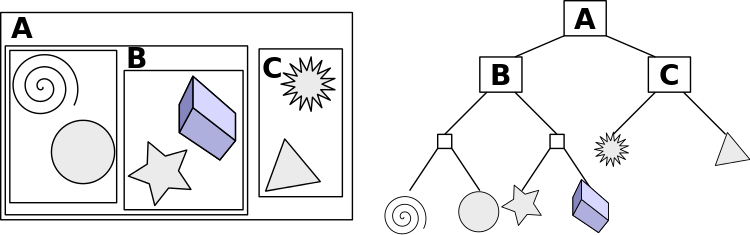
\includegraphics[keepaspectratio, width=\textwidth]{res/bvh.png}
    \end{figure}
    Все геометрические объекты, образующие листовые узлы дерева, заключены в эти BV.

    Затем эти узлы группируются в небольшие наборы и заключаются в более крупные BV.

\end{frame}

\begin{frame}
    \frametitle{Типы BV}
    \textbf{Типы ограничивающих объемов}:
    \begin{itemize}
        \item
            Sphere tree
        \item
            AABB tree (Axis Aligned Bounding Box)
        \item
            OBB tree (Oriented Bounding Box)
        \item
            k-DOP (Discrete Oriented Polytope)
        \item
            SSV (Swept Sphere Volume)
    \end{itemize}
    \begin{figure}
    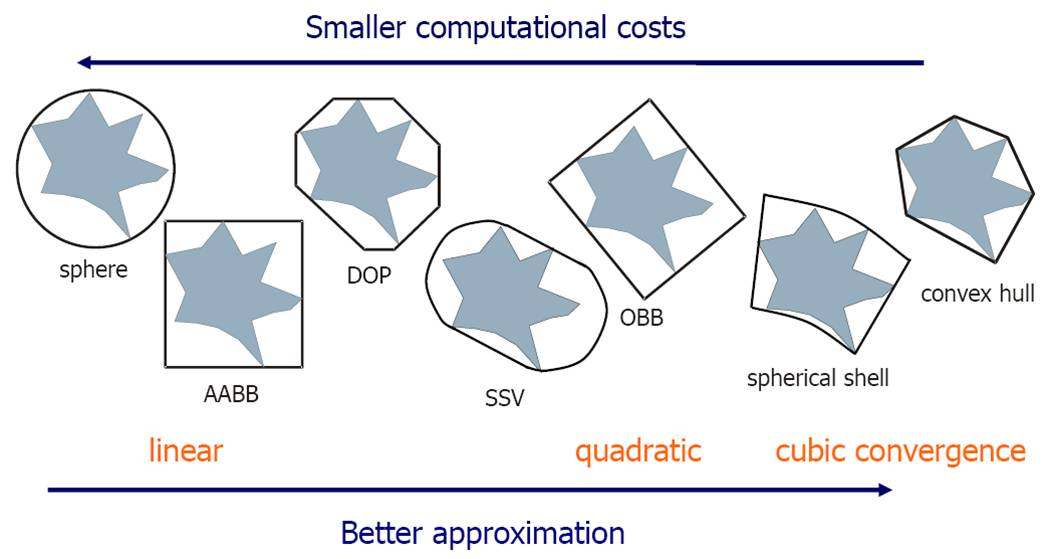
\includegraphics[keepaspectratio, width=\textwidth]{res/bvh_types.jpg}
    \end{figure}
\end{frame}

\begin{frame}
    \frametitle{BVH для трассировки лучей}
    \begin{block}{Зачем?}
        BVH часто используются в трассировке лучей для устранения потенциальных кандидатов
        на пересечение в сцене путем пропуска геометрических объектов,
        расположенных в ограничивающих объемах,
        которые не пересекаются текущим лучом.
    \end{block}
    Путем организации BV в BVH временная сложность (количество выполненных тестов)
    может быть уменьшена с линейной до логарифмической от количества примитивов (треугольников).

    В контексте ускоряющей структуры для рейтрейсинга используются:
    \begin{itemize}
        \item
            AABB (Axis Aligned Bounding Box)
        \item
            OBB (Oriented Bounding Box) \textit{(намного реже)}
    \end{itemize}


\end{frame}

\begin{frame}
    \frametitle{Метрики}
    \textbf{Для оценки эффективности BVH используются метрики}:
    \begin{itemize}
        \item
            Количество обойдённых узлов (NodesCount – NC)
        \item
            Количество обойдённых листьев (LeavesCount – LC)
        \item
            Кол-во арифметических операций проверки пересечения AABB (или др.) с лучом (AOC)
        \item
            Количество тестов луч-треугольник (или кол-во арифметических операций, TC)
        \item
            Количество длинных прыжков в пределах 1 буфера (LongJumpCount – LJC)
        \item
            Объём памяти, прочитанный (BusLoadInBytes – BLB)
        \item
            Leaf Count Variability (LCV)
        \item
            Время на определённом CPU
        \item
            Время на определённом GPU (не для всех)
        \item
            Общий объём памяти на всё дерево
    \end{itemize}
\end{frame}

\begin{frame}
    \frametitle{Функция стоимости BVH дерева}
    \begin{block}{Traversal cost \(c_T\) }
        Средняя стоимость пересечения луча c BV
    \end{block}
    \begin{block}{Intersection cost \(c_I\) }
        Средняя стоимость пересечения луча с примитивом сцены
    \end{block}
    \begin{block}{Conditional probability \(P(N_c\lvert N)\) }
        Условная вероятность пересечения дочернего узла \(N_c\) при пересеченном узле \(N\)
    \end{block}
    \begin{block}{Cost function}
        \(
        c(N) = \begin{cases}
            c_T + \displaystyle \sum_{N_c} P(N_c \lvert N)c(N_c)  \\
            c_I \lvert N \rvert\text{ \textit{(if N is leaf)} }
        \end{cases}
        \)
    \end{block}
\end{frame}

\begin{frame}
    \frametitle{Кэширование}
    \begin{block}{Cache locality CPU \& GPU}
        Когда вы обращаетесь к памяти, ее фрагменты кэшируются на разных уровнях.
        Локальность кеша относится к вероятности того,
        что последовательные операции будут находиться в кеше и,
        следовательно, будут выполняться быстрее.
    \end{block}
    \begin{block}{GPU Texture memory}
        Текстурная память GPU относится к аппаратному блоку, который мапается на глобальную память GPU.
        Этот аппаратный блок предоставляет свой механизм кэширования.
        \begin{itemize}
            \item
                максимизации 2D пространственной локальности
            \item
                аппаратная обработка адресов, выходящих за границы
        \end{itemize}
    \end{block}
\end{frame}

\begin{frame}
    \frametitle{Data layout}
    \begin{block}{Идея}
        Изменения порядка узлов и их внутреннего представления может улучшить \textbf{cache locality}
        и тем самым уменьшить \textbf{traversal cost}.
    \end{block}
\end{frame}

\begin{frame}
    \frametitle{Название слайда}
    \begin{itemize}
        \item
            a
        \item
            b
    \end{itemize}
\end{frame}

\end{document}
